\documentclass{beamer}
% \documentclass[handout]{beamer}

% \usetheme{Antibes}
% \usetheme{Berlin}
\usetheme{CambridgeUS}
% \usetheme{Copenhagen}

\usepackage{hyperref}
\usepackage{caption}
\usepackage{ytableau}
\usepackage{tikz-cd}
\usepackage{centernot}
\usepackage[shortlabels]{enumitem}
\usepackage{cases}
\usepackage{bbm}

\usepackage{booktabs}                
\usepackage{listings} % 코드 하이라이팅을 위해 추가

\usetikzlibrary{shadows}

\newtheorem{thm}{Theorem}[section]
\newtheorem{FermatLastTheorem}{Fermat's Last Theorem}[section]
\newtheorem{IMO_P2}{IMO 2024 Problem 2}[section]
\newtheorem{lem}[thm]{Lemma}
\newtheorem{prop}[thm]{Proposition}
\newtheorem{cor}[thm]{Corollary}
\newtheorem{conj}[thm]{Conjecture}
\newtheorem*{conj1}{Conjecture 1}
\newtheorem*{conj2}{Conjecture 2}
\newtheorem*{conj3}{Conjecture 3}
\theoremstyle{definition}
\newtheorem{exam}[thm]{Example}
\newtheorem{prob}[thm]{Problem}
\newtheorem{defn}[thm]{Definition}
\newtheorem{assumption}{Assumption}
\newtheorem{todo}{To-Do}
\newtheorem{remark}[thm]{Remark}

\newcommand\asc{\operatorname{asc}}
\newcommand\des{\operatorname{des}}
\newcommand\inv{\operatorname{inv}}
\newcommand\inc{\operatorname{inc}}
\newcommand\sgn{\operatorname{sgn}}
\newcommand\sh{\operatorname{sh}}
\newcommand\rk{\operatorname{rank}}
\newcommand\lex{\operatorname{lex}}
\newcommand\row{\operatorname{row}}
\newcommand\col{\operatorname{col}}
%% \newcommand\deg{\operatorname{deg}}
\newcommand\ch{\operatorname{ch}}
\newcommand\Red{\operatorname{Red}}
\newcommand\plac{\operatorname{plac}}
\newcommand\nCox{\operatorname{nCox}}

\newcommand\Des{\operatorname{Des}}
\newcommand\SYT{\operatorname{SYT}}
\newcommand\SSYT{\operatorname{SSYT}}
\newcommand\Par{\operatorname{Par}}
\newcommand\Comp{\operatorname{Comp}}

\newcommand\Ind{\operatorname{Ind}}

\newcommand\GL{\operatorname{GL}}
\newcommand\gl{\mathfrak{gl}}

\newcommand\NSym{\mathsf{NSym}}
\newcommand\Sym{\mathsf{Sym}}
\newcommand\QSym{\mathsf{QSym}}

\newcommand\gge{\succcurlyeq}
\newcommand\lle{\preccurlyeq}
\newcommand\trigeq{\unrhd}
\newcommand\trileq{\unlhd}

\newcommand\TT{\mathcal{T}}
\newcommand\UU{\mathcal{U}}
\newcommand\EE{\mathcal{E}}
\newcommand\SSS{\mathcal{S}}
\newcommand\II{\mathcal{I}}
\newcommand\LL{\mathcal{L}}
\newcommand\HH{\mathcal{H}}
\newcommand\SYM{\mathfrak{S}}

\newcommand\ZZ{\mathbb{Z}}
\newcommand\NN{\mathbb{N}}
\newcommand\QQ{\mathbb{Q}}
\newcommand\CC{\mathbb{C}}

\newcommand\xx{\mathbf{x}}
\newcommand\yy{\mathbf{y}}
\newcommand\uu{\mathbf{u}}
\newcommand\mm{\mathbf{m}}

\newcommand\ee{\mathfrak{e}}
\newcommand\hh{\mathfrak{h}}
\newcommand\ff{\mathfrak{f}}
\newcommand\sch{\mathfrak{s}}
\newcommand\pp{\mathfrak{p}}
\newcommand\mono{\mathfrak{m}}
\newcommand\FF{\mathfrak{F}}
\newcommand\MM{\mathfrak{M}}

\newcommand\ww{\mathsf{w}}
\newcommand\vv{\mathsf{v}}
\newcommand\zz{\mathsf{z}}

\newcommand\oo{\mathfrak{o}}

\newcommand\equivclass[1]{#1/{\sim}}
\newcommand\qand{\quad\mbox{and}\quad}
\newcommand\mand{\mbox{ \& }}
\newcommand{\precdot}{\prec\mathrel{\mkern-5mu}\mathrel{\cdot}}

\newcommand\CHK[1]{\textcolor{red}{#1}}
\newcommand\RED[1]{\textcolor{red}{#1}}
\newcommand\remph[1]{\emph{\textcolor{red}{#1}}}
\newcommand\bemph[1]{\emph{\textcolor{blue}{#1}}}

\title{FunSearch: doing mathematics via LLM}
\author[Team DM]{Team DM}
% \institute[KIAS]{KIAS}
\date[]{Winter School on Math+AI \\ \today}

%%%%%%%%%%%%%%%%%%%%%%%%%%%%%%%%%%%%%%%%%%%%%%

\AtBeginSection[]{%
\begin{frame}
    \tableofcontents[currentsection, subsectionstyle=show/show/hide]
\end{frame}
}

%%%%%%%%%%%%%%%%%%%%%%%%%%%%%%%%%%%%%%%%%%%%%%

\makeatletter
\let\save@measuring@true\measuring@true
\def\measuring@true{%
  \save@measuring@true
  \def\beamer@sortzero##1{\beamer@ifnextcharospec{\beamer@sortzeroread{##1}}{}}%
  \def\beamer@sortzeroread##1<##2>{}%
  \def\beamer@finalnospec{}%
}
\makeatother

%%%%%%%%%%%%%%%%%%%%%%%%%%%%%%%%%%%%%%%%%%%%%%

\makeatletter
\newenvironment<>{proofs}[1][\proofname]{%
    \par
    \def\insertproofname{#1\@addpunct{.}}%
    \usebeamertemplate{proof begin}#2}
  {\usebeamertemplate{proof end}}
\newenvironment<>{proofc}{%
  \setbeamertemplate{proof begin}{\begin{block}{}}
    \par
    \usebeamertemplate{proof begin}}
  {\usebeamertemplate{proof end}}
\newenvironment<>{proofe}{%
    \par
    \pushQED{\qed}
    \setbeamertemplate{proof begin}{\begin{block}{}}
    \usebeamertemplate{proof begin}}
  {\popQED\usebeamertemplate{proof end}}
\makeatother

%%%%%%%%%%%%%%%%%%%%%%%%%%%%%%%%%%%%%%%%%%%%%%

\begin{document}

\begin{frame}
  \titlepage
\end{frame}

\begin{frame}
  % \frametitle{AI for Math}
  \begin{center}
    \includegraphics[scale=.125]{./figures/AI4Math-diagram.png} \\
    Examples: AlphaGeometry, FunSearch, AlphaEvolve
  \end{center}
\end{frame}

\begin{frame}
  \frametitle{FunSearch}
  \begin{center}
    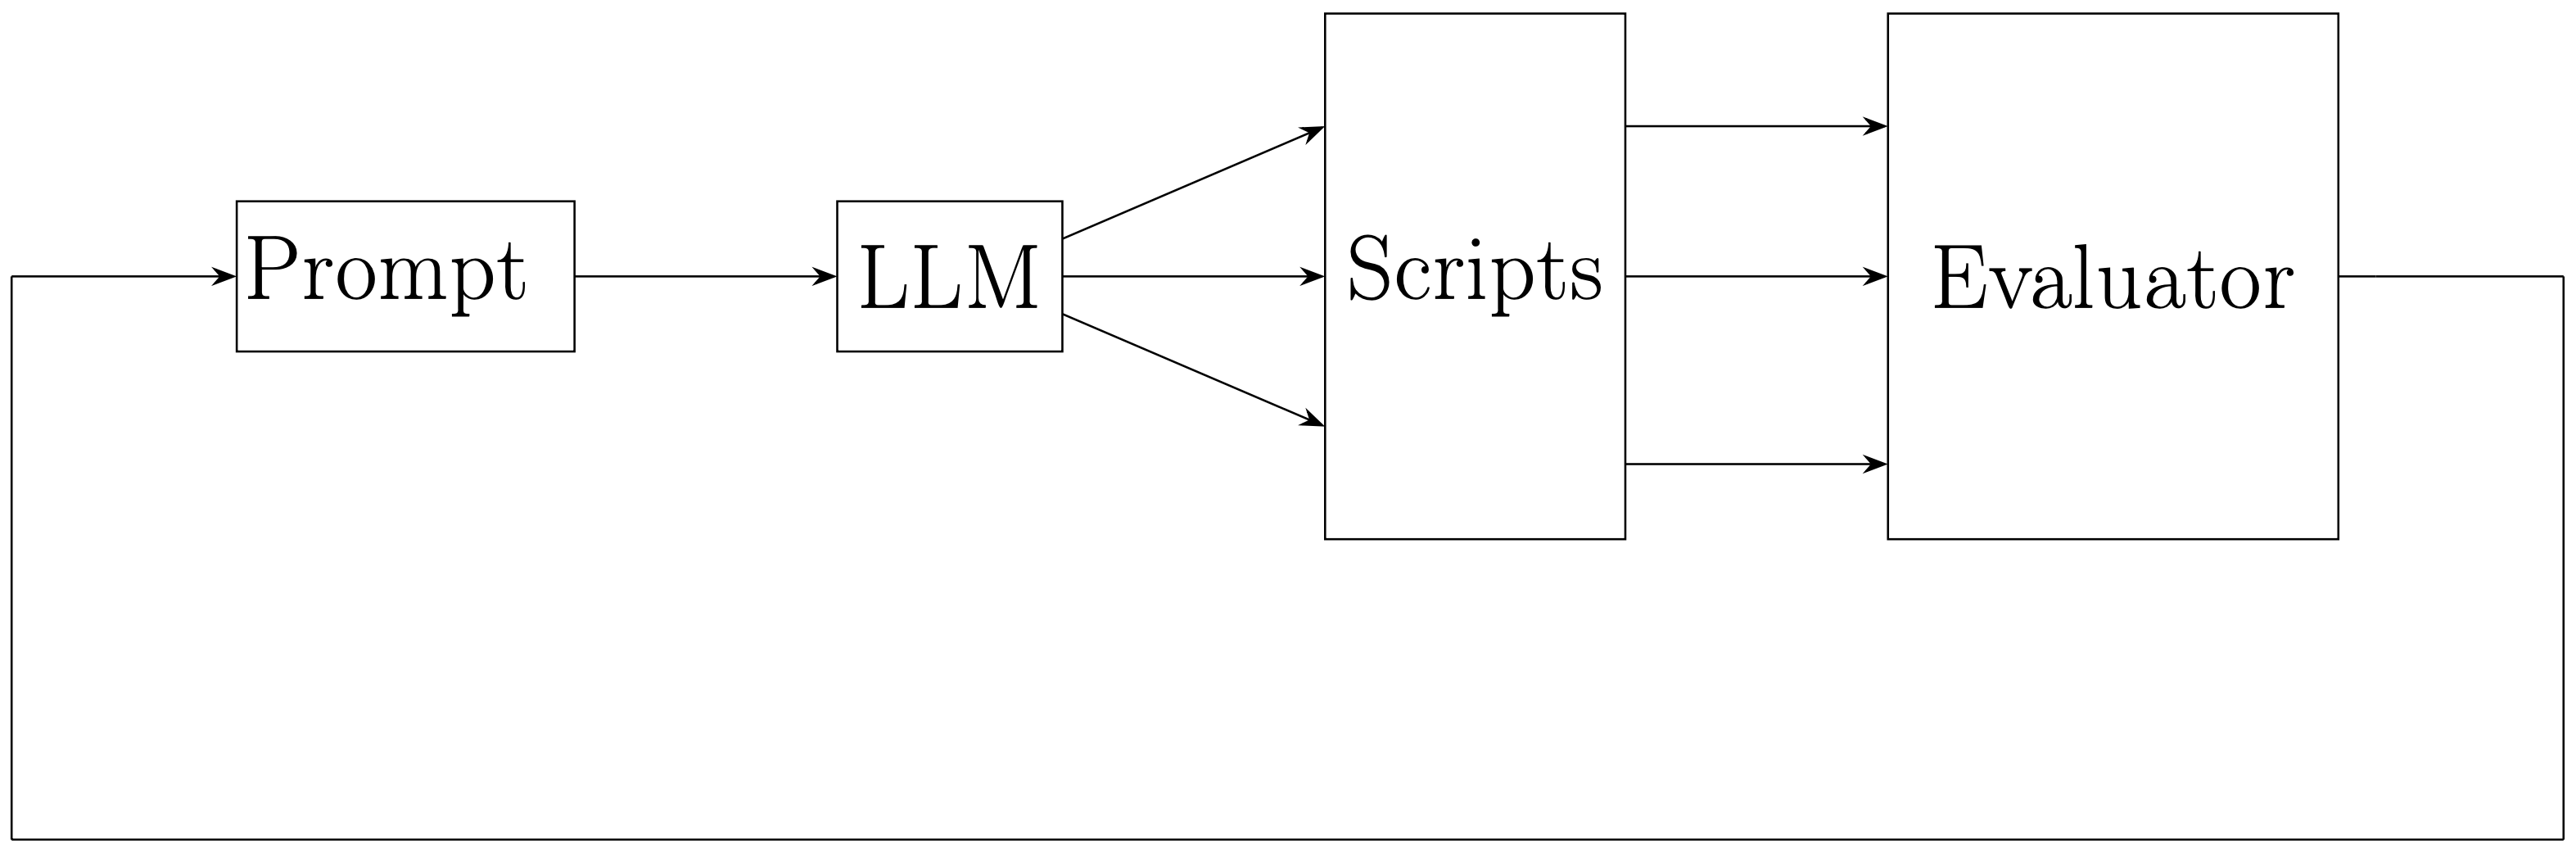
\includegraphics[scale=.2]{./figures/Workflow.png} \\
    FunSearch workflow (from \emph{Ellenberg et al. 2025})
  \end{center}
  \begin{enumerate}[label=(\roman*)]
  \item Generate candidate programs (Python functions).  
  \item Evaluate their performance on the target problem.  
  \item Feed the best (and diverse) candidates back to the LLM prompt.  
  \item The LLM produces new variants—forming the next generation.  
\end{enumerate}
\end{frame}

\begin{frame}
  \frametitle{What problems FunSearch can handle}
  \begin{itemize}
    \item Problems that are easy to evaluate but hard to solve directly. \vspace{.3cm}
    \item Especially suited for:
      \begin{itemize}
        \item[-] Extremal or additive combinatorics (e.g., Cap Set problem)
        \item[-] Number theory problems with clear scoring metrics
        \item[-] Combinatorial optimization (e.g., Bin packing)
      \end{itemize}
    \item FunSearch discovers \emph{heuristics or algorithms}, not full proofs.
  \end{itemize}
\end{frame}

\begin{frame}
  \frametitle{Problem 1: Cap Set problem}
  \begin{itemize}
    \item The \textbf{Cap Set problem}: find the largest subset of $(\mathbb{Z}/3\mathbb{Z})^n$ containing no three elements whose sum is zero. \vspace{.3cm}
    \item FunSearch discovered a new construction in dimension 8, producing a cap set of size 512—the largest known—improving the record for the first time in 20 years. \vspace{.3cm}
  \end{itemize}
\end{frame}

\begin{frame}
  \frametitle{Problem 1: Cap Set problem}
  \begin{center}
    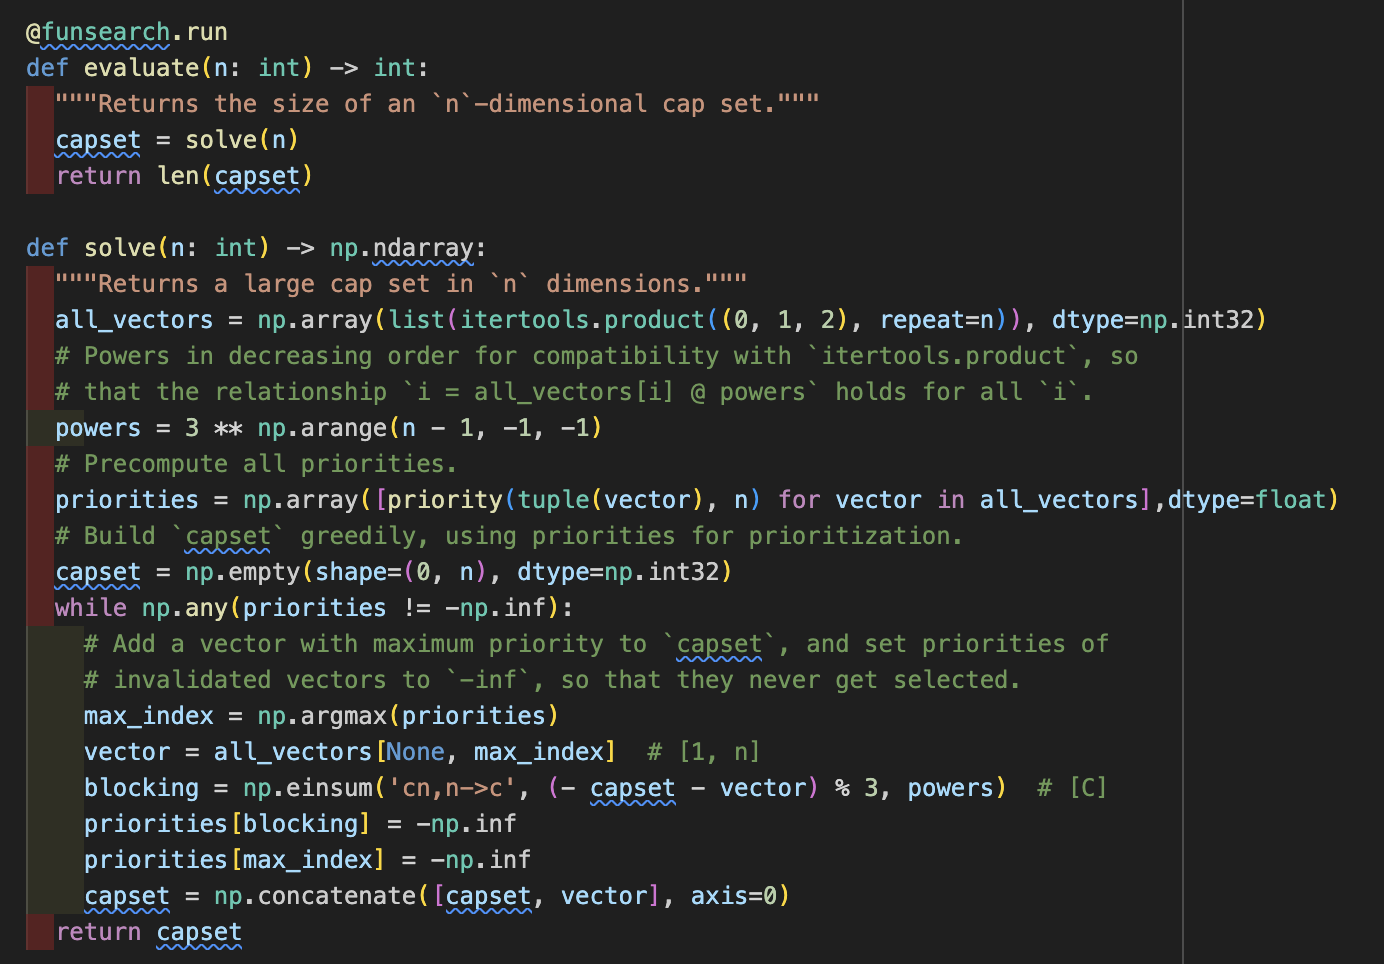
\includegraphics[scale=.4]{./figures/FunSearch_Eval_Solve.png}
  \end{center}
\end{frame}

\begin{frame}[fragile]
  \frametitle{Problem 1: Cap Set problem}
  \begin{block}{The priority function}
  \scriptsize
  \begin{verbatim}
  def priority(v: tuple[int, ...], n: int) -> float:
    """Returns the priority, as a floating point number, of the vector `v` of length `n`. The vector 'v' is a tuple of values in {0,1,2}.
      The cap set will be constructed by adding vectors that do not create a line in order by priority.
    """
    unique_elements = len(set(v))
    vector_magnitude = np.linalg.norm(v)
    balance_score = (3 - np.max(np.bincount(v, minlength=3))) / 3
    diversity_score = 1 - (unique_elements / 3)
    symmetry_score = np.sum(np.abs(np.bincount(v, minlength=3) - (len(v) / 3))) / len(v)
    stability_score = np.std(v) / 3
    evenness_score = 1 - (np.sum(np.square(np.bincount(v, minlength=3))) / (len(v) ** 2))
    compactness_factor = np.sum(v) / (3*n)
    return (unique_elements / n if n > 0 else 0.0) + vector_magnitude / n + balance_score + diversity_score + symmetry_score + stability_score + evenness_score - 0.5*compactness_factor  # Modified weight on compactness
  \end{verbatim}
  \normalsize
  The score of this priority function is 396. (The known best score is 512)
  \end{block}
\end{frame}

\begin{frame}[fragile]
  \frametitle{Problem 2: Hypergraph Tur\'{a}n problem}
  A \textbf{Tur\'{a}n problem} asks for the maximum number of edges in a graph/hypergraph that does not contain a specific forbidden subgraph.
  For a $3$-uniform hypergraph, we want to find the maximum number of edges $T(n, K_4^{(3)})$ in an $n$-vertex hypergraph with no four vertices spanning three edges (no $K_4^{(3)}$).
  \vspace{.3cm}

  For \( n=12 \), the known best result is 136.
\end{frame}

\begin{frame}[fragile]
  \frametitle{Problem 2: Hypergraph Tur\'{a}n problem}
  \begin{block}{The priority function}
  \scriptsize
  \begin{verbatim}
  def priority(p: tuple[int, int, int], n: int) -> float:
    """Returns the priority, as a floating point number, of the vector `p` of length `n`.
      The vector 'p' is a tuple of size 3 with values in {0,1,...,n-1}, with entries appearing in the increasing order.
      The hypergraph will be constructed by making crosses that do not create double crossings in order by priority.
    """
    mean_index = np.mean(p)
    distance = np.sum(np.abs(np.array(p) - mean_index))

    # Refine scaling to better represent spread and account for small adjustments
    scaling_factor = 1 + np.sqrt(distance + 1) * 0.5 + 0.05 * np.std(p)

    return (n / scaling_factor) * (1 + (mean_index / (n + 1))) + 0.01
  \end{verbatim}
  \normalsize
  This priority function constructs a 3-uniform hypergraph consisting of
  133 edges such that the hypergraph has no \( K_4^{(3)} \) as a subgraph.
  \end{block}
\end{frame}

\begin{frame}
  \frametitle{Problem 3: The Ramsey number}
  % ** EXPLAIN WHAT THE RAMSEY NUMBER IS **
  The \textbf{Ramsey number} $R(s, t)$ is the minimum number of vertices $N$ such that any edge coloring of the complete graph $K_N$ with two colors (say, red and blue) contains a monochromatic red clique of size $s$ or a blue clique of size $t$.
  \vspace{.3cm}

  Note that
  \[
    R(4,4) = 18,
  \]
  that is, every edge coloring of \( K_{18} \) with red and blue has a monochromatic
  clique of size 4 (in red or blue).
\end{frame}

\begin{frame}[fragile]
  \frametitle{Problem 3: The Ramsey number}
  \scriptsize
  \begin{verbatim}
  BOOST_DEG_REDUCED = 0.1
  BOOST_UNIQUE = 0.5
  def priority(e: tuple[int, int, int], n: int) -> float:
      """n: the size of the vertex set
          e: the tuple (i, j, c) where (i, j) is an edge which lies in the vertex set and c is 0 (red) or 1 (blue).
          This function returns the priority, as a floating point number, of the "color-assigned edge" e.
          The graph, which is a subgraph of K_n, will be constructed by adding colored edges that do not create a monochromatic K_4 in order by priority.
      """
      i, j, c = e
      priority = 0.0

      if c in [0, 1]:
          priority += BOOST_UNIQUE

      priority += BOOST_DEG_REDUCED * (3 - np.random.uniform(0, 0.5))  # Limited range for variability
      return priority
  \end{verbatim}
  \normalsize
  This priority function gives an edge-coloring of \( K_{14} \) without a monochromatic clique of size 4.
\end{frame}

\begin{frame}[fragile]
  \frametitle{Problem 3: The Ramsey number}
  \begin{center}
    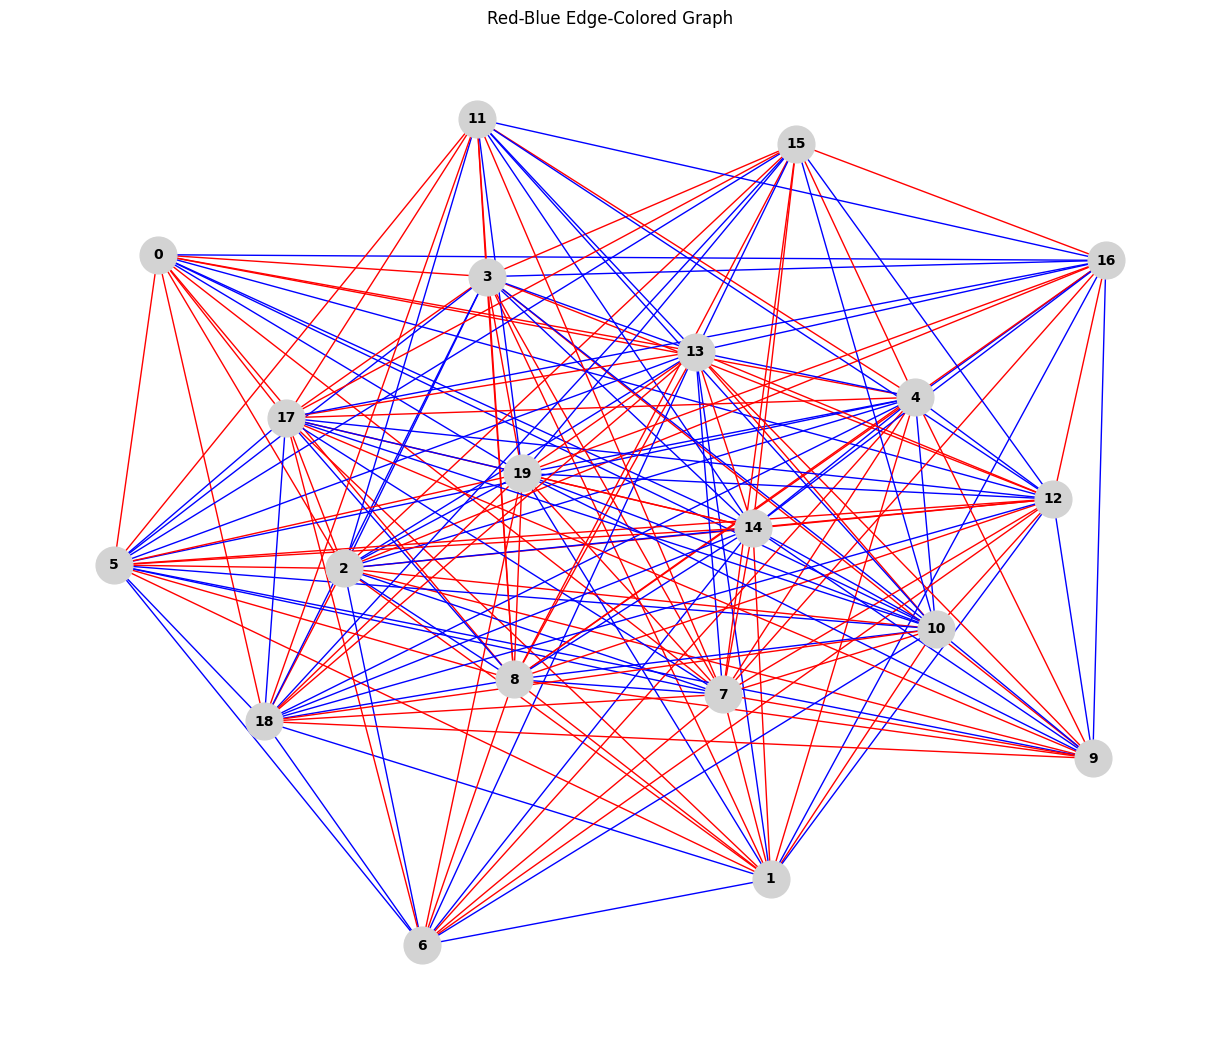
\includegraphics[scale=.3]{./figures/r44-14.png}
  \end{center}
\end{frame}

\begin{frame}[fragile]
  \frametitle{Problem 4: Meandric permutation}
  A \textbf{meander} is a non-intersecting closed curve that intersects a straight line multiple times.

  \begin{center}
    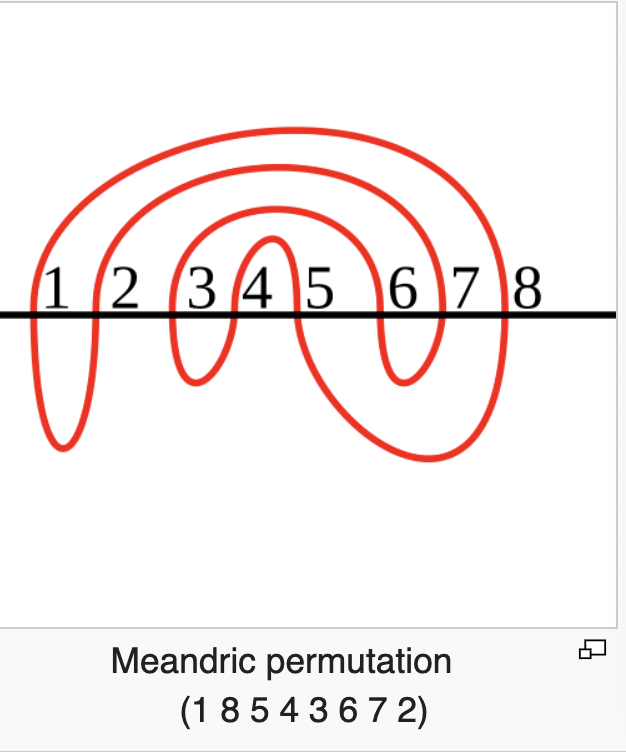
\includegraphics[scale=.33]{./figures/meander.png}
  \end{center}

  \vspace{.3cm}

  A characterization of whether a given permutation is a Meandric permutation
  is unknown.
\end{frame}

\begin{frame}[fragile]
  \frametitle{Problem 4: Meandric permutation}
  \scriptsize
  \begin{verbatim}
  def priority(v: Tuple[int, ...], n: int) -> float:
    """Returns the priority (a real-valued score) of the permutation `v` of length 2n.
        The search will try to modify this function so that:
          * true Meandric permutations tend to have score > 0
          * non-Meandric permutations tend to have score <= 0
    """
    mid = n + 1

    consecutive_count = sum(1 for i in range(len(v)-1) if abs(v[i]-v[i+1]) == 1)
    parity_score = sum(1 for i in range(1, 2 * n+1) if v[i-1] % 2 == i % 2)
    unique_pairs = sum(1 for i in range(1, n+1)
        if (v[2*(i-1)], v[2*(i-1)+1]) in itertools.permutations([i, i+n]))

    alternating_score = sum(1 for i in range(2*n-1)
        if (v[i] % 2) != (v[i+1] % 2))
    
    total_score = (consecutive_count+parity_score+unique_pairs+alternating_score) / (3*n+mid)
    return (total_score*2)-1  # Normalize to range [-1, 1]
  \end{verbatim}
\end{frame}

\begin{frame}[fragile]
  \frametitle{Problem 5: CFR algorithm}
  % ** EXPLAIN WHAT THE CFR ALGORITHM is **
  \textbf{CFR (Counterfactual Regret Minimization)} is an iterative algorithm used to find a Nash equilibrium in imperfect-information games (like poker) by minimizing regret over time.
  \vspace{.3cm}

  We've tried to find a better algorithm by modifying the CFR algorithm.
\end{frame}

\begin{frame}[fragile]
  \frametitle{Problem 5: CFR algorithm}
  \scriptsize
  \begin{verbatim}
  def update_regret(player: int, t: int, R_prev: np.ndarray, 
            sigma_hist_A: np.ndarray, sigma_hist_B: np.ndarray) -> np.ndarray:
    R = R_prev.astype(float)
    p, q = float(sigma_hist_A[-1]), float(sigma_hist_B[-1])
    adv = _adv_A(q) if player == 0 else _adv_B(p)
    R += np.maximum(adv, 0.0) + (THRESH if player == 1 else 0)
    return np.clip(R, EPS, None) 
  \end{verbatim}
  \normalsize
  The algorithm based on the above function seems to be better than
  the CFR algorithm, but...
\end{frame}

\begin{frame}[fragile]
  \frametitle{Other applications}                
  Furthermore, we've applied FunSearch to various other problems:
  \begin{itemize}
    \item[$\bullet$] halving pseudoline problem
    \item[$\bullet$] finding a long path on permutations
    \item[$\bullet$] characterization of the dinv statistics on Dyck paths
    \item[$\bullet$] finding a pattern on Kronecker coefficients
    \item[$\bullet$] finding a large set of Jones polynomials
  \end{itemize}
\end{frame}

\section*{}
\begin{frame}
\begin{center}
\Huge{Thank you}
\end{center}
\end{frame}

\end{document}